\subsection{その他のミニアプリ関連プロジェクト}
\label{sec:その他のミニアプリ}

海外においてもFIBERと同様にミニアプリを整備して性能評価用の共通情報資源
として活用しようとする動向がある。

\subsubsection{米国のミニアプリ関連 - CORALプロジェクト}
米国においては米国エネルギー省の管轄下にある
Argonne国立研究所、Lawrence Livermore国立研究所、Oak Ridge国立研究所の
3研究所のHPC調達共通化にともない、性能評価用に用いられるCORALベンチマーク
が公開されている\cite{CORAL-benchmarks,CORAL-slides}。
CORALベンチマークの内 LSMS, CAM-SE, QMCPACK, NAMD を除き、アプリは基本的に
ミニアプリである。

\begin{table}[H]
%	\begin{table}[htb]
\caption{CORAL benchmarks \(tier1およびtier2 アプリのみ掲載\)}
\label{tab:CORAL-apps-names}
{
%\tiny
%\scriptsize
%\footnotesize
%\small
%\normalsize
\begin{tabular}{p{75mm}|p{75mm}} \hline
%	\begin{tabular}{l|l} \hline
アプリ名 &	CORALによるジャンル分け \\ \hline \hline
LSMS, QBOX, HACC, Nekbone
	& Scalable Science Benchmarks
	\\ \hline
CAM-SE, UMT2013, AMG2013, MCB, QMCPACK, NAMD, LULESH, SNAP, miniFE
	& Throughput Benchmarks
	\\ \hline
Graph500, Integer Sort, Hash, SPECint2006
	& Data-Centric Benchmarks
	\\ \hline
CLOMP, IOR, CORAL MPI, STREAM, STRIDE, LCALS
	& Skeleton Benchmarks
	\\ \hline
\end{tabular}
}
\end{table}

\iffalse
\begin{table}[H]
\caption{CORAL benchmarks \(tier1およびtier2 アプリのみ掲載\)}
\label{tab:CORAL-apps-groups}
{
\begin{tabular}{p{50mm}|p{100mm}} \hline
CORALによるジャンル分け	& アプリ名  \\ \hline \hline
Scalable Science Benchmarks
	& LSMS, QBOX, HACC, Nekbone  \\ \hline
Throughput Benchmarks
	& CAM-SE, UMT2013, AMG2013, MCB, QMCPACK, NAMD, LULESH,
	  SNAP, miniFE  \\ \hline
Data-Centric Benchmarks
	& Graph500, Integer Sort, Hash, SPECint2006  \\ \hline
Skeleton Benchmarks
	& CLOMP, IOR, CORAL MPI, STREAM, STRIDE, LCALS  \\ \hline
\end{tabular}
}
\end{table}
\fi

これらのミニアプリ全体で以下の計算負荷を網羅するように選択されている。

%	\begin{table}[htb]
\begin{table}[H]
\caption{CORAL benchmarks Platform Stress Areas}
\label{tab:CORAL-benchmarks-stress}
{
\begin{tabular}{p{30mm}|p{120mm}} \hline
%	\begin{tabular}{l|l} \hline
システムの部位	&	注目する主な計算負荷 \\ \hline \hline

計算コア
	& 浮動小数点演算、SIMD/ベクトル化、整数・分岐処理 \\
%	& Floating point intensive	\\
%	& SIMD/vectorization	\\
%	& Integer/branch	\\
	\hline
メモリアクセス
	& メモリバンド幅、連続・等間隔アクセス、不連続アクセス、大規模メモリ領域\\
%	&	Memory bandwidth	\\
%	&	Regular(strided) memory access	\\
%	&	Irregular memory access	\\
%	&	Large memory footprint	\\
	\hline
ノード間通信
	& 非局所的P2P通信、短いメッセージ、長いメッセージ、集合通信、
		バイセクションバンド幅 \\
%	&	Non-local P2P communication	\\
%	&	Small messages	\\
%	&	Large messages	\\
%	&	Collective communication	\\
%	&	Bisection bandwidth	\\
	\hline
スレッド処理
	& 細粒度スレッド処理 \\
%	&	Fine grain threading	\\
	\hline
\end{tabular}
}
\end{table}


\subsubsection{米国のミニアプリ関連 - MANTEVOプロジェクト}
また、米国においてはコデザインを推進するためのミニアプリの開発整備それ自体に
主眼をおいたプロジェクトの試みもあり、
ミニアプリを用いた性能モデリングと実際のプラットフォームにおける
挙動とのマッピングが2009年あたりから提唱されている。
MANTEVOプロジェクトはそのようなプロジェクトの一つである\cite{MANTEVO-project}。
MANTEVOプロジェクトの特徴として、ミニアプリの開発整備は全てフルアプリの
開発者が行っていることがあげられる。
以下に Workshop on Representative Applications 2015 \cite{MANTEVO-Reps}
において紹介されたMANTEVO3.0ミニアプリのリストを示す。


%	\begin{table}[htb]
\begin{table}[H]
\caption{MANTEVO 3.0 miniApp}
\label{tab:MANTEVO-miniapp}
{
\begin{tabular}{p{50mm}|p{100mm}} \hline
アプリ名		&	計算内容 \\ \hline

Cleverleaf 	&	Eulerian on structured grid with AMR  \\ \hline
CloverLeaf 	&	Compressible Euler eqns,explicit 2nd order accurate \\ \hline
CoMD 		&	Molecular dynamics(SPaSM)  \\ \hline
EpetraBenchmarkTest	&	Exercises Epetra sparse and dense kernels \\ \hline
HPCCG 		&	Unstructured implicit finiteelement  \\ \hline
miniFE 		&	Implicit finite element solver \\ \hline
miniGhost 	&	FDM/FVM explicit (haloexchangefocus) \\ \hline
miniMD 		&	Molecular dynamics(Lennard-Jones)  \\ \hline
miniXyce 	&	SPICE-style circuit simulator \\ \hline
miniAMR 		&	Adaptive mesh refinement of an Eulerian mesh \\ \hline
miniSMAC2D 	&	FD 2D incompressible N/S on a structured grid. \\ \hline
PathFinder 	&	Signature search \\ \hline
miniAero 	&	3D unstr FV R-K4th order time, inviscid Roe Flux \\ \hline
TeaLeaf 	&	Solid mechanics \\ \hline
\end{tabular}
}
\end{table}


\subsubsection{ヨーロッパのミニアプリ関連 - European Exascaleプロジェクト}
ヨーロッパにおいては2013年から2016年にかけて
European Exascale Projects (FP7)の活動の中で整備されたアプリケーションが
プロトアプリと称されているが、これらはミニアプリと同じ位置づけである。
Mini-FEM, BPMF, ExaMD, OASIS3-MCT の各プロトアプリが公開されている\cite{EXA2CT}。

%	\begin{table}[htb]
\begin{table}[H]
\caption{EXA2CT proto apps}
\label{tab:exa2ct-proto-apps}
{
\begin{tabular}{p{50mm}|p{100mm}} \hline
アプリ名		&	計算内容 \\ \hline
\hline
Mini-FEM & reproducing the assembly step of 3D FEM unstructured meshes \\ \hline
BPMF	& A big data and machine learning proto application \\ \hline
ExaMD	& A scalable proto-app library for Molecular Dynamics using
			the Adaptive Midpoint method  \\ \hline
OASIS3-MCT & Coupling code by CERFACS, developed for climate applications
\\ \hline
\end{tabular}
}
\end{table}


% 参考文献
%	\nocite{*}
%	\bibliographystyle{\rmbibstyle}
%	\bibliography{3-3}


\subsection{2章アプリケーションとミニアプリの対応}
\label{sec:apps-and-miniapps}

公開されている Fiberミニアプリ と サンプルデータを用いて計算を行った場合の
B/F値、および必要メモリ量を、2章アプリケーション要求性能値
{\textcolor{blue}{この表refはどこ?}} %\ref{}
に重ねた図を図\ref{fig:apps-miniapps} に示す。

\begin{figure}[h]
%	\centering
%	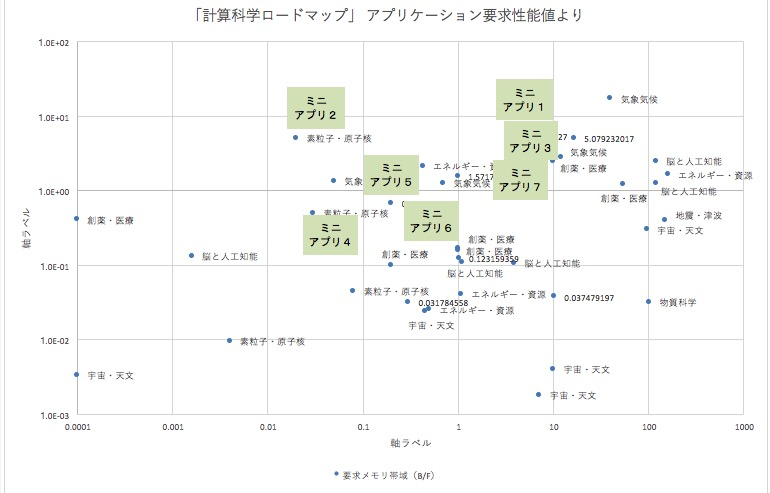
\includegraphics[clip]{figs/3-2-miniapps.jpg}
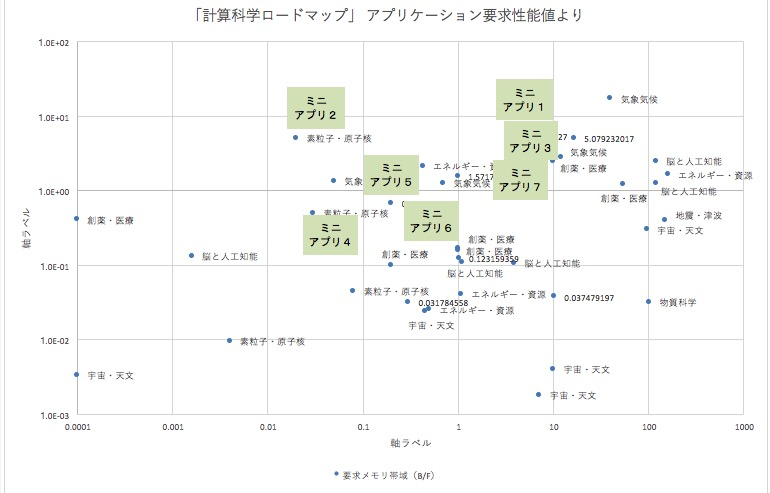
\includegraphics[width=\textwidth]{figs/3-2-miniapps.jpg}
\caption{2章アプリケーションとミニアプリの対応}
\label{fig:apps-miniapps}
\end{figure}

